\documentclass[
10pt, % Main document font size
letterpaper, % Paper type, use 'letterpaper' for US Letter paper
oneside, % One page layout (no page indentation)
%twoside, % Two page layout (page indentation for binding and different headers)
headinclude,footinclude, % Extra spacing for the header and footer
BCOR5mm, % Binding correction
]{scrartcl}

%%%%%%%%%%%%%%%%%%%%%%%%%%%%%%%%%%%%%%%%%
% Arsclassica Article
% Structure Specification File
%
% This file has been downloaded from:
% http://www.LaTeXTemplates.com
%
% Original author:
% Lorenzo Pantieri (http://www.lorenzopantieri.net) with extensive modifications by:
% Vel (vel@latextemplates.com)
%
% License:
% CC BY-NC-SA 3.0 (http://creativecommons.org/licenses/by-nc-sa/3.0/)
%
%%%%%%%%%%%%%%%%%%%%%%%%%%%%%%%%%%%%%%%%%

%----------------------------------------------------------------------------------------
%	REQUIRED PACKAGES
%----------------------------------------------------------------------------------------

\usepackage[
nochapters, % Turn off chapters since this is an article        
beramono, % Use the Bera Mono font for monospaced text (\texttt)
eulermath,% Use the Euler font for mathematics
pdfspacing, % Makes use of pdftex’ letter spacing capabilities via the microtype package
dottedtoc % Dotted lines leading to the page numbers in the table of contents
]{classicthesis} % The layout is based on the Classic Thesis style

\usepackage{arsclassica} % Modifies the Classic Thesis package

\usepackage[T1]{fontenc} % Use 8-bit encoding that has 256 glyphs

\usepackage[utf8]{inputenc} % Required for including letters with accents

\usepackage{graphicx} % Required for including images
\graphicspath{{Figures/}} % Set the default folder for images

\usepackage{enumitem} % Required for manipulating the whitespace between and within lists

\usepackage{subfig} % Required for creating figures with multiple parts (subfigures)

\usepackage{amsmath,amssymb,amsthm} % For including math equations, theorems, symbols, etc

\usepackage{varioref} % More descriptive referencing

%----------------------------------------------------------------------------------------
%	THEOREM STYLES
%---------------------------------------------------------------------------------------

\theoremstyle{definition} % Define theorem styles here based on the definition style (used for definitions and examples)
\newtheorem{definition}{Definition}

\theoremstyle{plain} % Define theorem styles here based on the plain style (used for theorems, lemmas, propositions)
\newtheorem{theorem}{Theorem}

\theoremstyle{remark} % Define theorem styles here based on the remark style (used for remarks and notes)

%----------------------------------------------------------------------------------------
%	HYPERLINKS
%---------------------------------------------------------------------------------------

\hypersetup{
%draft, % Uncomment to remove all links (useful for printing in black and white)
colorlinks=true, breaklinks=true, bookmarks=true,bookmarksnumbered,
urlcolor=webbrown, linkcolor=RoyalBlue, citecolor=webgreen, % Link colors
pdftitle={}, % PDF title
pdfauthor={\textcopyright}, % PDF Author
pdfsubject={}, % PDF Subject
pdfkeywords={}, % PDF Keywords
pdfcreator={pdfLaTeX}, % PDF Creator
pdfproducer={LaTeX with hyperref and ClassicThesis} % PDF producer
} % Include the structure.tex file which specified the document structure and layout
\usepackage{amsmath}
\title{\normalfont{Fluid Simulation on CUDA GPUs}}
\subtitle{Johns Hopkins University: EN.605.617.81.SP23 Introduction to GPU Programming }
\author{\spacedlowsmallcaps{Nate Lao (nlao1@jh.edu)}}
\date{May 7th 2023}

\begin{document}
\maketitle

\section{Summary} %%%%%%%%%%%%%%%%%%%%%%%%%%%%%%%%%%%%%%%%%%%%%%%%%%%%%%%%%%%%%%%%%%%%%%%%%%%%%%%%%%%%%%%%%%%%%%%%%%%%%%%%%%%%%%%%%%%%%%%%
The Simulation of Fast Fluid Dynamics project is an implementation of 2-dimensional fluid computation on NVIDIA GPUs leveraging the CUDA library.
The algorithms in this project were largely based on the whitepaper presented in

\begin{center}
    \href{https://developer.nvidia.com/gpugems/gpugems/part-vi-beyond-triangles/chapter-38-fast-fluid-dynamics-simulation-gpu}{GPU GEMS - Chapter 38}
\end{center}

The source code for this project is publicly available on GitHub. At the time of writing, version 0.1.0 is the referenced baseline:

\begin{center}
    \url{https://github.com/naterjlao/cuda_fluidsim}
\end{center}

The report is an overall summary of design decisions, implementation details and limitations presented in this project.
\begin{figure}[h]
    \centering
    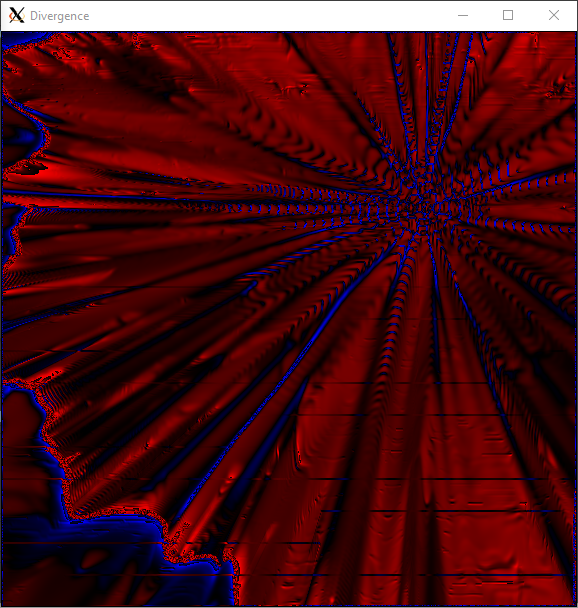
\includegraphics[scale=0.5]{../png/divergence_example.PNG}
    \caption{Fluid Divergence Field}
\end{figure}

\pagebreak
\section{Technologies} %%%%%%%%%%%%%%%%%%%%%%%%%%%%%%%%%%%%%%%%%%%%%%%%%%%%%%%%%%%%%%%%%%%%%%%%%%%%%%%%%%%%%%%%%%%%%%%%%%%%%%%%%%%%%%%%%%%%%%%%
This project was developed on a Linux/Debian machine with a NVIDIA RTX 3060 GPU. There is no guarantee that the source code will be compatible
with other systems. Appropriate modifications may need to be performed in order to build this project on other systems.

The main driver of this project is the NVIDIA CUDA library, the version information for CUDA nvcc compiler is as follows:
\begin{verbatim}
    $ nvcc --version
    nvcc: NVIDIA (R) Cuda compiler driver
    Copyright (c) 2005-2022 NVIDIA Corporation
    Built on Mon_Oct_24_19:12:58_PDT_2022
    Cuda compilation tools, release 12.0, V12.0.76
    Build cuda_12.0.r12.0/compiler.31968024_0
\end{verbatim}

OpenCV was used to render visual representations of fluid calculations and to provide iteractivity for the user. The version information is
presented below:

\begin{verbatim}
    OpenCV version : 3.2.0
    Major version : 3
    Minor version : 2
    Subminor version : 0
\end{verbatim}

The machine that executes the simulation does not need a desktop environment. X-Forwarding may be used to project visual renders on a client
machine.

\section{Data Structures} %%%%%%%%%%%%%%%%%%%%%%%%%%%%%%%%%%%%%%%%%%%%%%%%%%%%%%%%%%%%%%%%%%%%%%%%%%%%%%%%%%%%%%%%%%%%%%%%%%%%%%%%%%%%%%%%%%%%%%%%
The scope of this project will only deal with a 2-dimensional field for fluid simulation. The data structures are defined tailored to 2-dimensions,
however the code may be modified to accommodate 3-dimensions. These data structures are desinged with the CUDA architecture in mind, to simplify
the development process and to provide an optimization to processing.

Three types of datastructures are used:
\begin{itemize}
    \item Vector Field Matrix
    \item Scalar Field Matrix
    \item BGRA Matrix
\end{itemize}

\subsection{Vector Field Matrix}
The Vector Field Matrix is represented as multidimensions array in memory. The allocation of this matrix is equivalent to the following declaration:
\begin{center}
    \begin{verbatim}
        float v_field[y-dim][x-dim][2]
    \end{verbatim}
\end{center}
In this declaration, \verb|y-dim| and \verb|x-dim| are the number of elements in the $y$ (rows) and $x$ (column) dimensions in terms of pixels, respectively.
The \verb|2| constant represents the individual vector component for each pixel the 0-index is x-component and 1-index is the y-component.

This would be represented in memory as follows:
\begin{center}
    $v\_field = \begin{bmatrix}
        (0.0,0.0) & (0.0,0.0) & (0.0, 0.0)\\
        (0.0,0.0) & (0.0,0.0) & (0.0, 0.0)\\
        (0.0,0.0) & (2.0,3.0) & (0.0, 0.0)\\
    \end{bmatrix}$
\end{center}

In this example, accessing the following indices in C would the following:
\begin{center}
    \begin{verbatim}
        v_field[2][1][0] -> 2.0
        v_field[2][1][1] -> 3.0
    \end{verbatim}
\end{center}

Deriving the array index given an x and y coordinate and vector component index is as follows:
\begin{equation}
    index = (y * x_{dim} + x) * 2 + CI_{vector}
\end{equation}

\subsection{Scalar Field Matrix}
The Scalar Field Matrix is similar to the Vector Field Matrix. The declaration of this data structure is more straightforward to its vector counterpart:
\begin{verbatim}
    float s_field[y-dim][x-dim]
\end{verbatim}
Deriving the array index given an x and y coordinate is as follows:
\begin{equation}
    index = y * x_{dim} + x
\end{equation}
    
\subsection{BGRA}
The BGRA (Blue-Green-Red-Alpha) Matrix is a representation of color channel intensities for each pixel. In OpenCV, each channel is represented
an an octet byte, where \verb|0x00| is the minimal intensity and \verb|0xFF| is the maximum.

For the designed architecture, a little-endian system is used. The byte order for every pixel is arranged as follows:
\begin{center}
    \begin{verbatim}
        pixel = 0xAARRGGBB
    \end{verbatim}
\end{center}

\pagebreak
\section{Algorithms} %%%%%%%%%%%%%%%%%%%%%%%%%%%%%%%%%%%%%%%%%%%%%%%%%%%%%%%%%%%%%%%%%%%%%%%%%%%%%%%%%%%%%%%%%%%%%%%%%%%%%%%%%%%%%%%%%%%%%%%%
jfkljflkdjlk


\pagebreak
\section{Limitations} %%%%%%%%%%%%%%%%%%%%%%%%%%%%%%%%%%%%%%%%%%%%%%%%%%%%%%%%%%%%%%%%%%%%%%%%%%%%%%%%%%%%%%%%%%%%%%%%%%%%%%%%%%%%%%%%%%%%%%%%
jfkljflkdjlk

\end{document}